\chapter{Конструкторский раздел}

Конструкторская часть содержит рассмотрение архитектуры разрабатываемого программного комплекса, структуры собственного протокола передачи данных между частями комплекса, а также основные алгоритмы, используемые в отдельных частях комплекса.

\section{Архитектура программного комплекса}
Разрабатываемый программный комплекс должен придерживаться модели взаимодействия «клиент» - «сервер». Таким образом, в программном комплексе дифференцируются две части. 

Серверная часть отвечает за соединение игроков и обмен информацией между клиентами. 

Клиентская часть передает серверу данные о себе и получает данные от сервера во время игры. Клиенты могут взаимодействовать друг с другом только посредством серверной коммуникации, т.е. если клиент желает отправить данные другому клиенту, из этих данных вначале формируется пакет, соответствующий разработанному для обмена информацией протоколу, затем этот пакет отправляется серверу, и уже сервер пересылает его конечному получателю.

\section{Протокол взаимодействия}

Типы сообщений Т:
\begin{enumerate}
\item FINISH - закончить игру
\item START - начать игру
\item RECEIVE NAME - получить имя
\item SEND NAME - отправить имя
\item NEW BALL - новый мяч
\item ARR BALL - массив мячей
\item FLIPPER TRIGGERED - движение рычага, координата пружины, счет
\end{enumerate}

\subsection{Пакеты сообщения}

Пакет NEW BALL новый мяч:
\begin{enumerate}
\item x - координата x;
\item y - координата y;
\item speedX - скорость по x;
\item speedY - скорость по y;
\item rotation - угол поворота;
\end{enumerate}

Пакет ARR BALL масив мячей:
\begin{enumerate}
\item количество элементов;
\item сами элементы:
  \begin{enumerate}
  \item x - координата x;
  \item y - координата y;
  \item rotation - угол поворота;
  \end{enumerate}
\end{enumerate}

Пакет FLIPPER TRIGGERED  движение рычага:
\begin{enumerate}
\item left - автивен левый;
\item right - автивен правый;
\item spring - координата пружины;
\item score - счет;
\end{enumerate}

\section{Алгоритм серверной части}

Сервер построен по типу <<thread per game session>>, т.е. для каждой игровой сессии создается новый поток. Т.е. сервер состоит из потоков добавления, соединения и потоков сессий. 

\subsection{Поток добавления}

Имеется массив ожидающих игроков. При появлении соединения, новый сокет добавляется в массив ожидающих игроков.

\subsection{Поток соединения}

Если количество элементов в массиве ожидающих игроков больше одного, то взять два последних элемента, соединить их в пару, удалить из массива ожидающих игроков. Запустить поток сессии для этой пары игроков.  

\subsection{Поток сессии}

В паре игроков имеем два сокета (К1 и К2), через которые сервер будет общаться с этими двумя клиентами.

Последовательность действий сервера:
\begin{enumerate}
\item отправить сообщение START К1
\item отправить сообщение START К2
\item получить подтверждение от К1 и К2 о начале игры;
\item получить имена от К1 и К2;
\item отправить имя соперника К1 и К2;
\item для каждого К1 и К2, пока не получено сообщение о завершении игры:
	\begin{enumerate}
	\item получить тип сообщения Т;
	\item получить структуру информации для типа Т и отправить её сопернику;
	\end{enumerate}
\item отправить сообщение FINISH сопернику
\end{enumerate} 

\section{Алгоритм клиентской части}

Клиент может находится в одном из состояний:
\begin{enumerate}
\item CREATE - только создан,
\item CONNECT- подлючен к серверу,
\item ACTIVE - идет игра,
\item FINISH - закончена игра,
\item END - отправлено сообщение о конце игры
\end{enumerate}

Последовательность действий клиента:
\begin{enumerate}
\item создать соединение с сервером,
\item поздороваться с соперником:
  \begin{enumerate}
  \item получить сообщение о старте игры;
  \item отправить своё имя;
  \item получить имя соперника;
  \end{enumerate}
\item пока состояние игрока - ACTIVE и пока не получено сообщение о завершении игры:
  \begin{enumerate}
  \item получить тип сообщения Т;
  \item получить структуру информации для типа Т;
  \end{enumerate}
\item отправить сообщение FINISH
\end{enumerate}

\subsection{Интерфейс взаимодейстия для клиента}

На клиенте могут быть вызвны следующие операции:
\begin{enumerate}
\item createConnection - создать соединение,
\item handshake - поздороваться с соперником,
\item setFinish - закончить игру,
\item getOpponentName - взять имя соперника,
\item getNewBall - взять новый шар соперника
\item getArrBallsOpponent - взять массив шаров соперника
\item getFlipperTriggered - взять информацию о рычаге соперника
\item sendArrBalls  - отправить массив своих шаров
\item sendNewBall - отправить свой новый шар
\item sendFlipperTriggered - отправить информацию о своем рычаге и счете
\end{enumerate}

\section{Схема}

\begin{figure}[h]
  \centering
  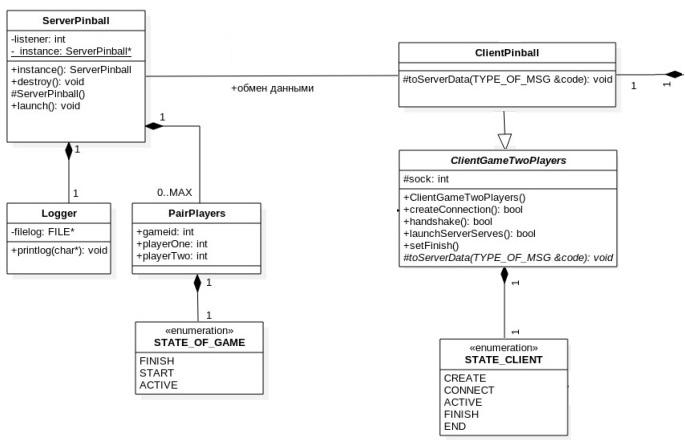
\includegraphics[width=\textwidth]{cs-diag.png}
  \caption{Диаграмма классов клиента и сервера.}
\end{figure}

\section{Выводы}
В данном разделе были рассмотрены архитектура разрабатываемого программного комплекса, структура пакетов собственного протокола обмена данными, а также основные алгоритмы взаимодействия и обмена данными между клиентом и сервером.